The patterns discussed here are a subset of the parallel patterns described in the book Structured Parallel Programming by McCool et al. We do not cover the patterns related to types of parallelism (e.g., fork-join, branchand-bound) but focus on the algorithmic patterns most useful for writing data-parallel kernels.\par

We wholeheartedly believe that understanding this subset of parallel patterns is critical to becoming an effective DPC++ programmer. The table in Figure 14-1 presents a high-level overview of the different patterns, including their primary use cases, their key attributes, and how their attributes impact their affinity for different hardware devices.\par

\hspace*{\fill} \par %插入空行
Figure 14-1. Parallel patterns and their affinity for different device 
types
% Please add the following required packages to your document preamble:
% \usepackage[normalem]{ulem}
% \useunder{\uline}{\ul}{}
\begin{table}[H]
	\begin{tabular}{|l|l|l|l|}
		\hline
		\textbf{Pattern}                                           & \textbf{Useful For}                                                        & \textbf{Key Attributes}                                                            & \textbf{Device Affinity}                                          \\ \hline
		Map                                                        & \begin{tabular}[c]{@{}l@{}}Simple parallel\\ kernels\end{tabular}          & \begin{tabular}[c]{@{}l@{}}No data dependences and\\ high scalability\end{tabular} & All                                                               \\ \hline
		Stencil                                                    & \begin{tabular}[c]{@{}l@{}}Structured data\\ dependences\end{tabular}      & \begin{tabular}[c]{@{}l@{}}Data dependences and\\ data re-use\end{tabular}         & \begin{tabular}[c]{@{}l@{}}Depends on stencil\\ size\end{tabular} \\ \hline
		Reduction                                                  & \begin{tabular}[c]{@{}l@{}}Combining partial\\ results\end{tabular}        & Data dependences                                                                   & All                                                               \\ \hline
		\begin{tabular}[c]{@{}l@{}}Scan\\ Pack/Unpack\end{tabular} & \begin{tabular}[c]{@{}l@{}}Filtering and\\ restructuring data\end{tabular} & Limited scalability                                                                & \begin{tabular}[c]{@{}l@{}}Depends on\\ problem size\end{tabular} \\ \hline
	\end{tabular}
\end{table}

\hspace*{\fill} \par %插入空行
\textbf{Map}

The map pattern is the simplest parallel pattern of all and will be immediately familiar to readers with experience of functional programming languages. As shown in Figure 14-2, each input element of a range is independently mapped to an output by applying some function. Many data-parallel operations can be expressed as instances of the map pattern (e.g., vector addition).\par

\hspace*{\fill} \par %插入空行
Figure 14-2. Map pattern
\begin{center}
	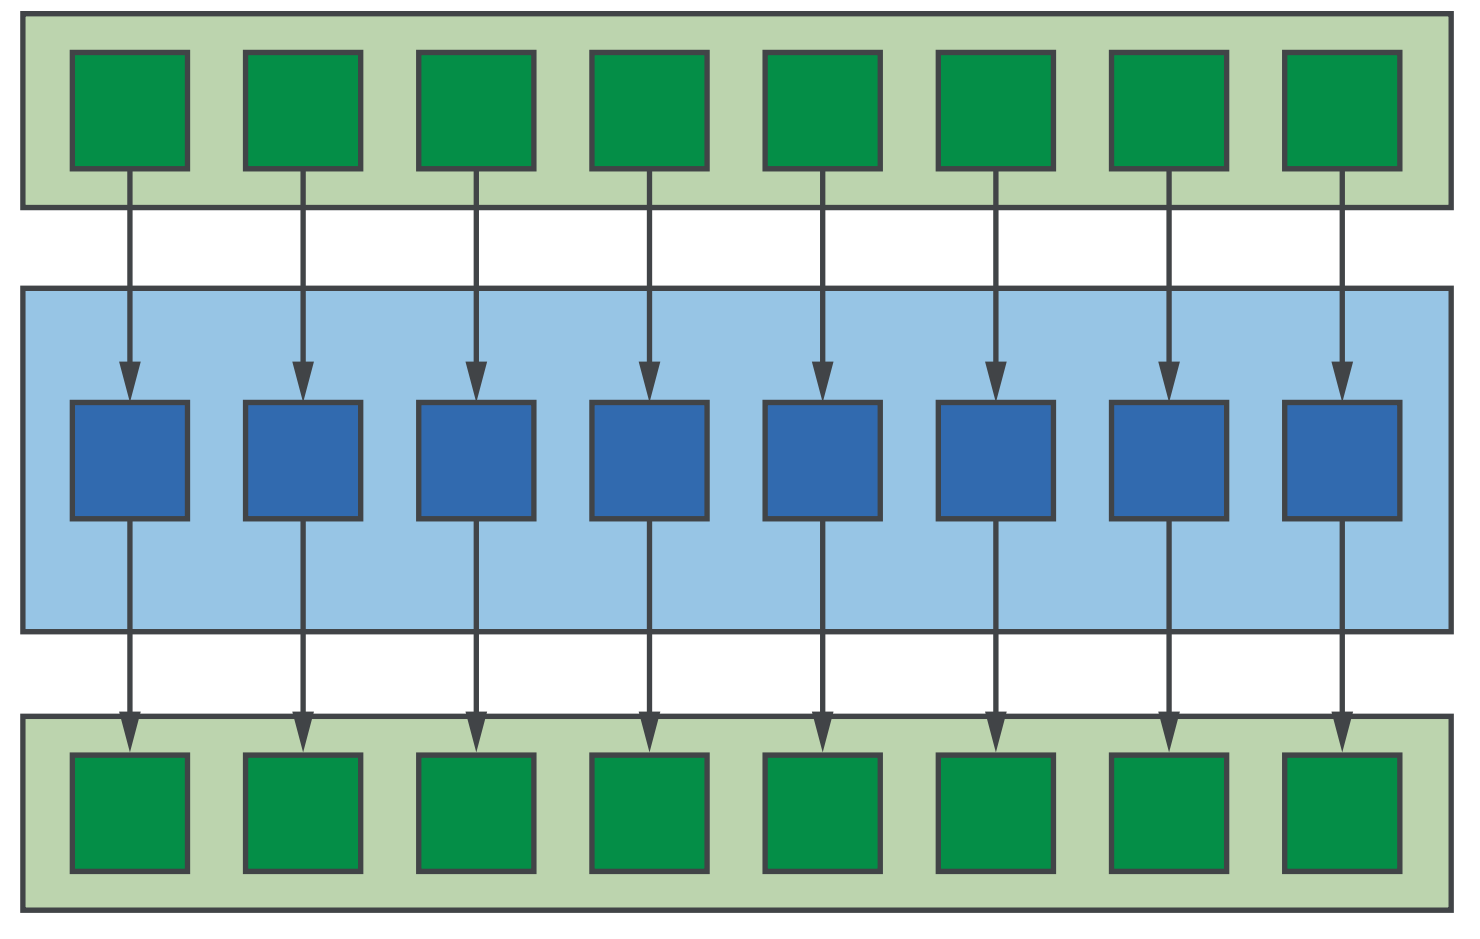
\includegraphics[width=1.\textwidth]{content/chapter-14/images/2}
\end{center}

Since every application of the function is completely independent, expressions of map are often very simple, relying on the compiler and/or runtime to do most of the hard work. We should expect kernels written to the map pattern to be suitable for any device and for the performance of those kernels to scale very well with the amount of available hardware parallelism.\par

However, we should think carefully before deciding to rewrite entire applications as a series of map kernels! Such a development approach is highly productive and guarantees that an application will be portable to a wide variety of device types but encourages us to ignore optimizations that may significantly improve performance (e.g., improving data reuse, fusing kernels).\par

\hspace*{\fill} \par %插入空行
\textbf{Stencil}

The stencil pattern is closely related to the map pattern. As shown in Figure 14-3, a function is applied to an input and a set of neighboring inputs described by a stencil to produce a single output. Stencil patterns appear frequently in many domains, including scientific/engineering applications (e.g., finite difference codes) and computer vision/machine learning applications (e.g., image convolutions).\par

\hspace*{\fill} \par %插入空行
Figure 14-3. Stencil pattern
\begin{center}
	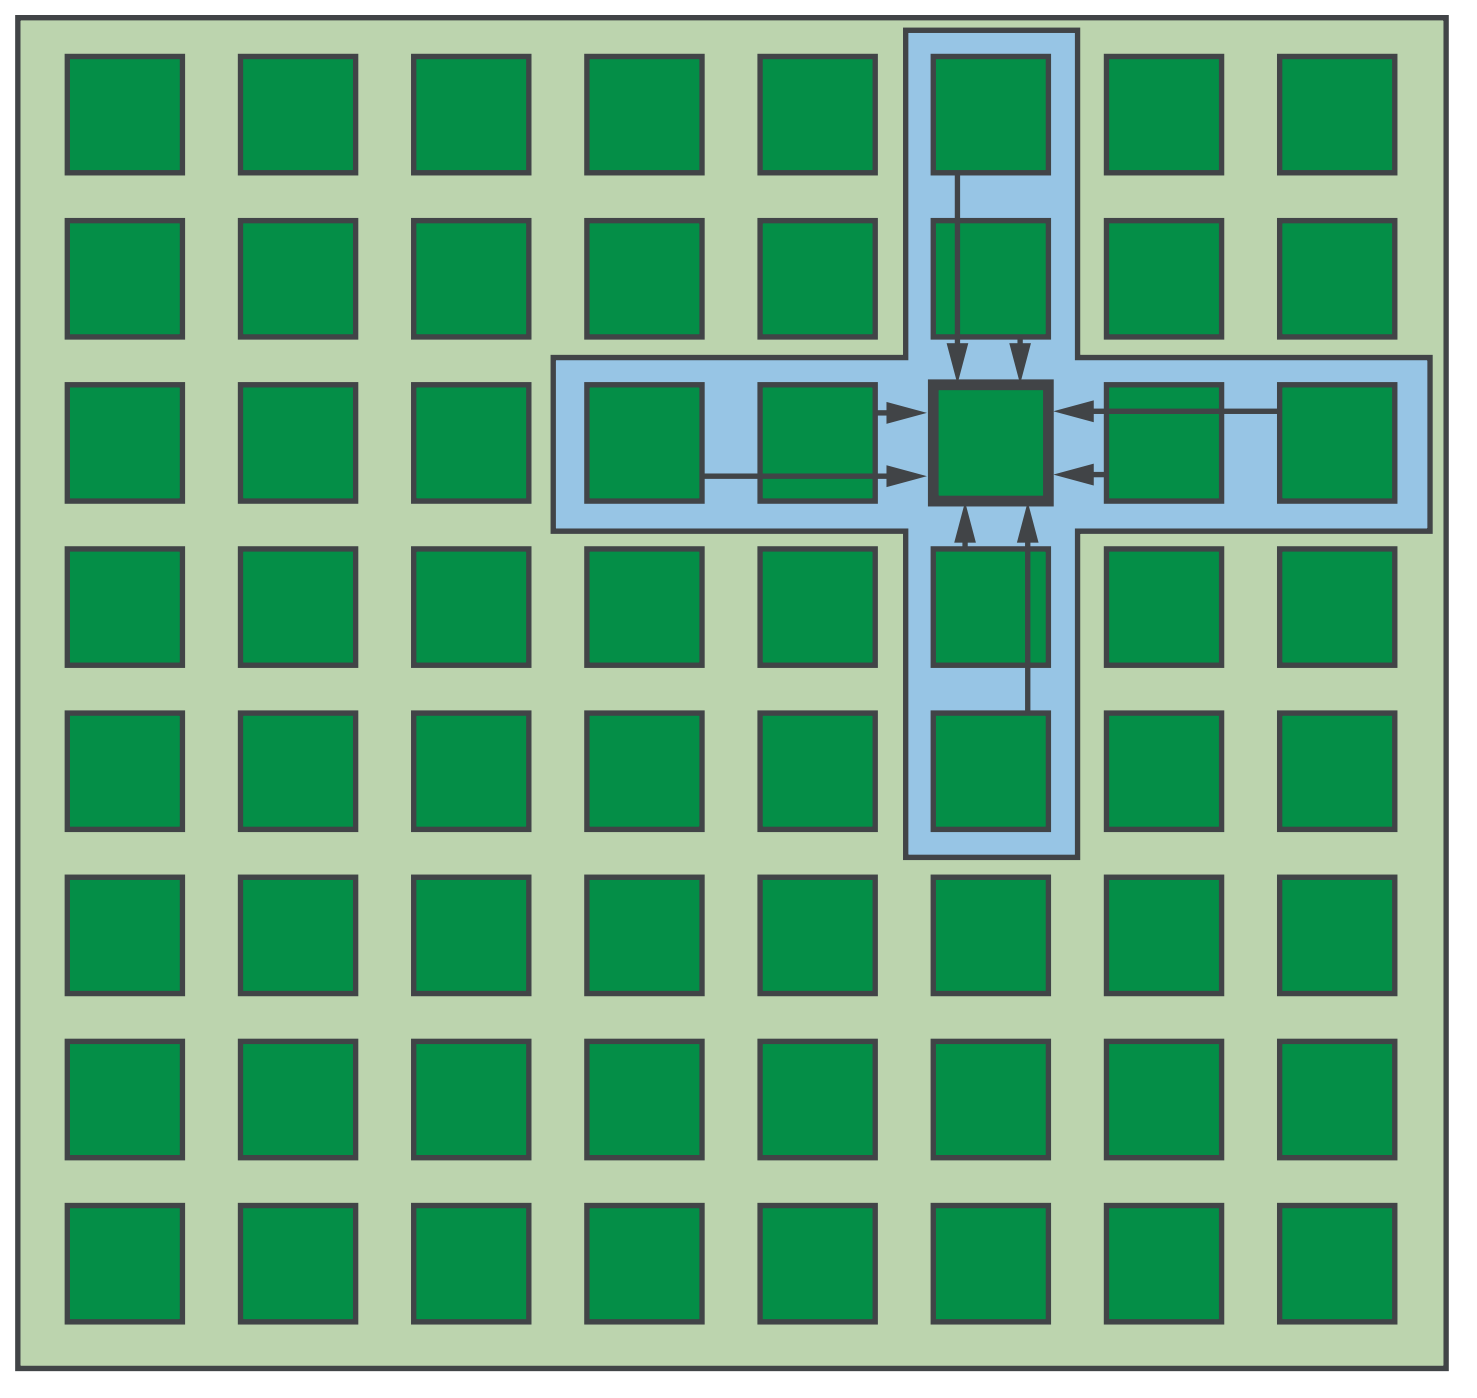
\includegraphics[width=1.\textwidth]{content/chapter-14/images/3}
\end{center}

When the stencil pattern is executed out-of-place (i.e., writing the outputs to a separate storage location), the function can be applied to every input independently. Scheduling stencils in the real world is often more complicated than this: computing neighboring outputs requires the same data, and loading that data from memory multiple times will degrade performance; and we may wish to apply the stencil in-place (i.e., overwriting the original input values) in order to decrease an application’s memory footprint.\par

The suitability of a stencil kernel for different devices is therefore highly dependent on properties of the stencil and the input problem. As a rule of thumb:\par

\begin{itemize}
	\item Small stencils can benefit from the scratchpad storage of GPUs.
	\item Large stencils can benefit from the (comparatively) large caches of CPUs.
	\item Small stencils operating on small inputs can achieve significant performance gains via implementation as systolic arrays on FPGAs.
\end{itemize}

Since stencils are easy to describe but complex to implement efficiently, stencils are one of the most active areas of domain-specific language (DSL) development. There are already several embedded DSLs leveraging the template meta-programming capabilities of C++ to generate high-performance stencil kernels at compile time, and we hope that it is only a matter of time before these frameworks are ported to DPC++.\par

\hspace*{\fill} \par %插入空行
\textbf{Reduction}

A reduction is a common parallel pattern which combines partial results from each instance of a kernel invocation using an operator that is typically associative and commutative (e.g., addition). The most ubiquitous examples of reductions are computing a sum (e.g., while computing a dot product) or computing the minimum/maximum value (e.g., using maximum velocity to set time-step size).\par

\hspace*{\fill} \par %插入空行
Figure 14-4. Reduction pattern
\begin{center}
	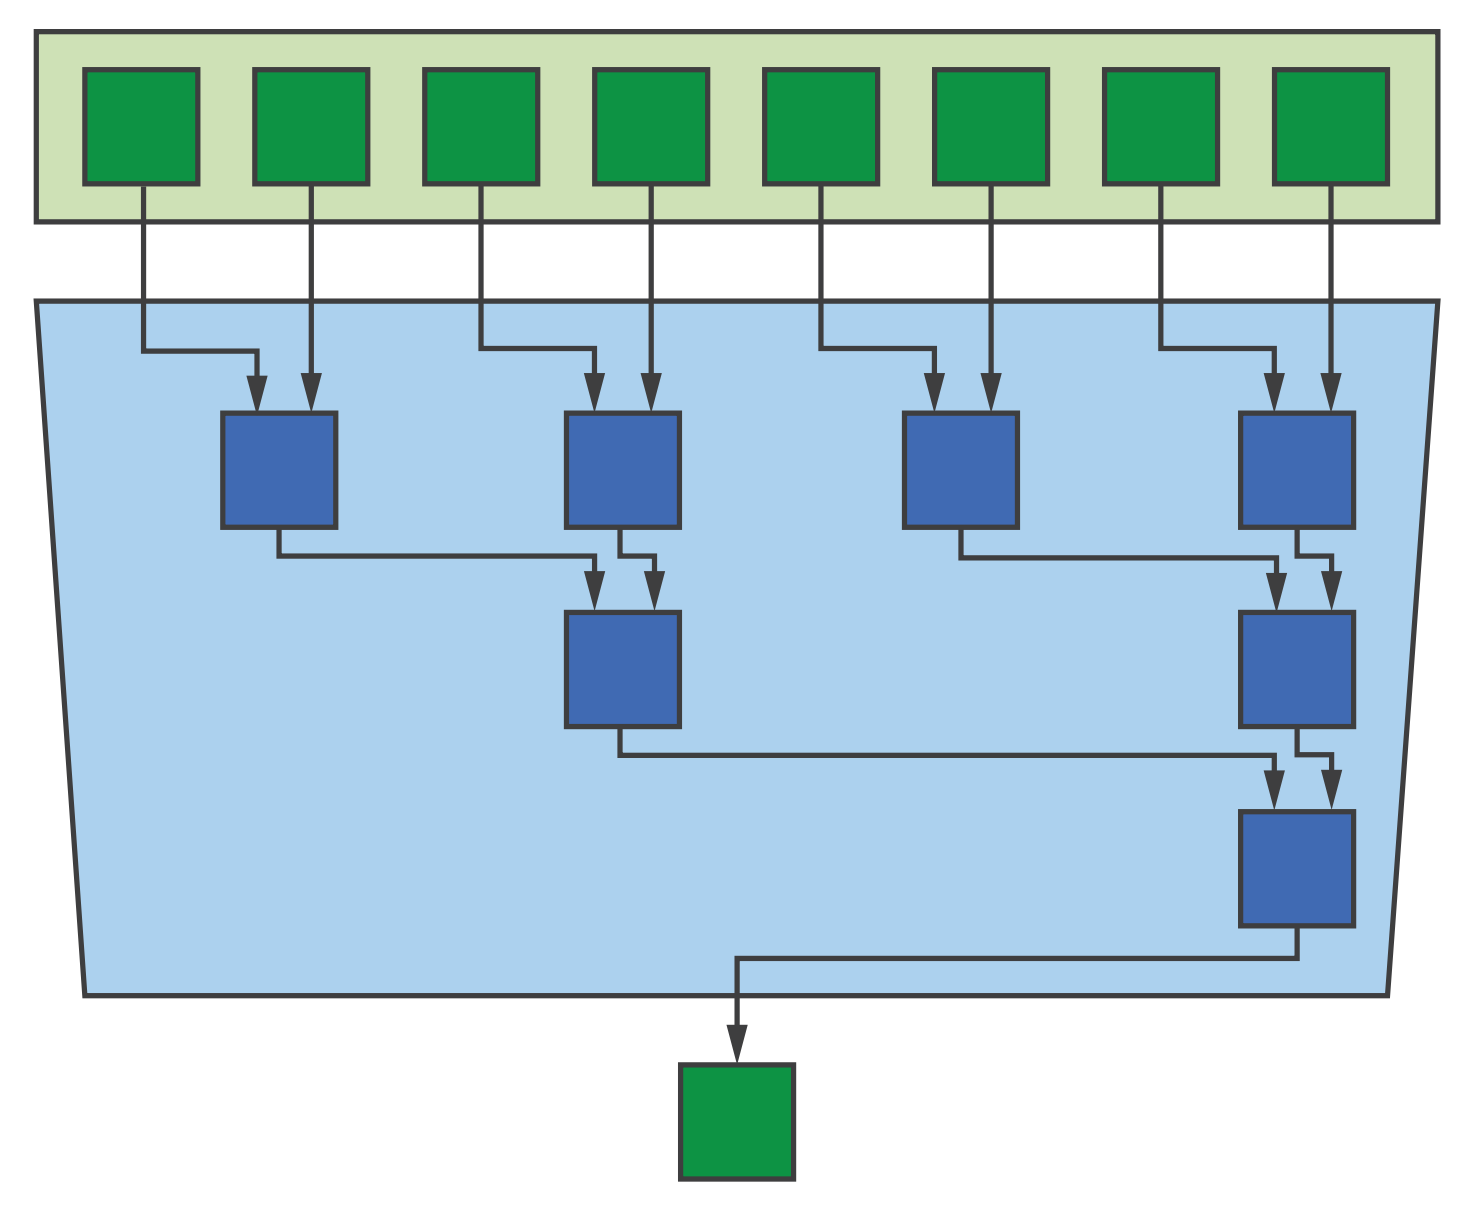
\includegraphics[width=1.\textwidth]{content/chapter-14/images/4}
\end{center}

Figure 14-4 shows the reduction pattern implemented by way of a tree reduction, which is a popular implementation requiring log2(N) combination operations for a range of N input elements. Although tree reductions are common, other implementations are possible—in general, we should not assume that a reduction combines values in a specific order.\par

Kernels are rarely embarrassingly parallel in real life, and even when they are, they are often paired with reductions (as in MapReduce frameworks) to summarize their results. This makes reductions one of the most important parallel patterns to understand and one that we must be able to execute efficiently on any device.\par

Tuning a reduction for different devices is a delicate balancing act between the time spent computing partial results and the time spent combining them; using too little parallelism increases computation time, whereas using too much parallelism increases combination time.\par

It may be tempting to improve overall system utilization by using different devices to perform the computation and combination steps, but such tuning efforts must pay careful attention to the cost of moving data between devices. In practice, we find that performing reductions directly on data as it is produced and on the same device is often the best approach. Using multiple devices to improve the performance of reduction patterns therefore relies not on task parallelism but on another level of data parallelism (i.e., each device performs a reduction on part of the input data).\par

\hspace*{\fill} \par %插入空行
\textbf{Scan}

The scan pattern computes a generalized prefix sum using a binary associative operator, and each element of the output represents a partial result. A scan is said to be inclusive if the partial sum for element i is the sum of all elements in the range [0, i] (i.e., the sum including i). A scan is said to be exclusive if the partial sum for element i is the sum of all elements in the range [0, i]) (i.e., the sum excluding i).\par

At first glance, a scan appears to be an inherently serial operation, since the value of each output depends on the value of the previous output! While it is true that scan has less opportunities for parallelism than other patterns (and may therefore be less scalable), Figure 14-5 shows that it is possible to implement a parallel scan using multiple sweeps over the same data.\par

\hspace*{\fill} \par %插入空行
Figure 14-5. Scan pattern
\begin{center}
	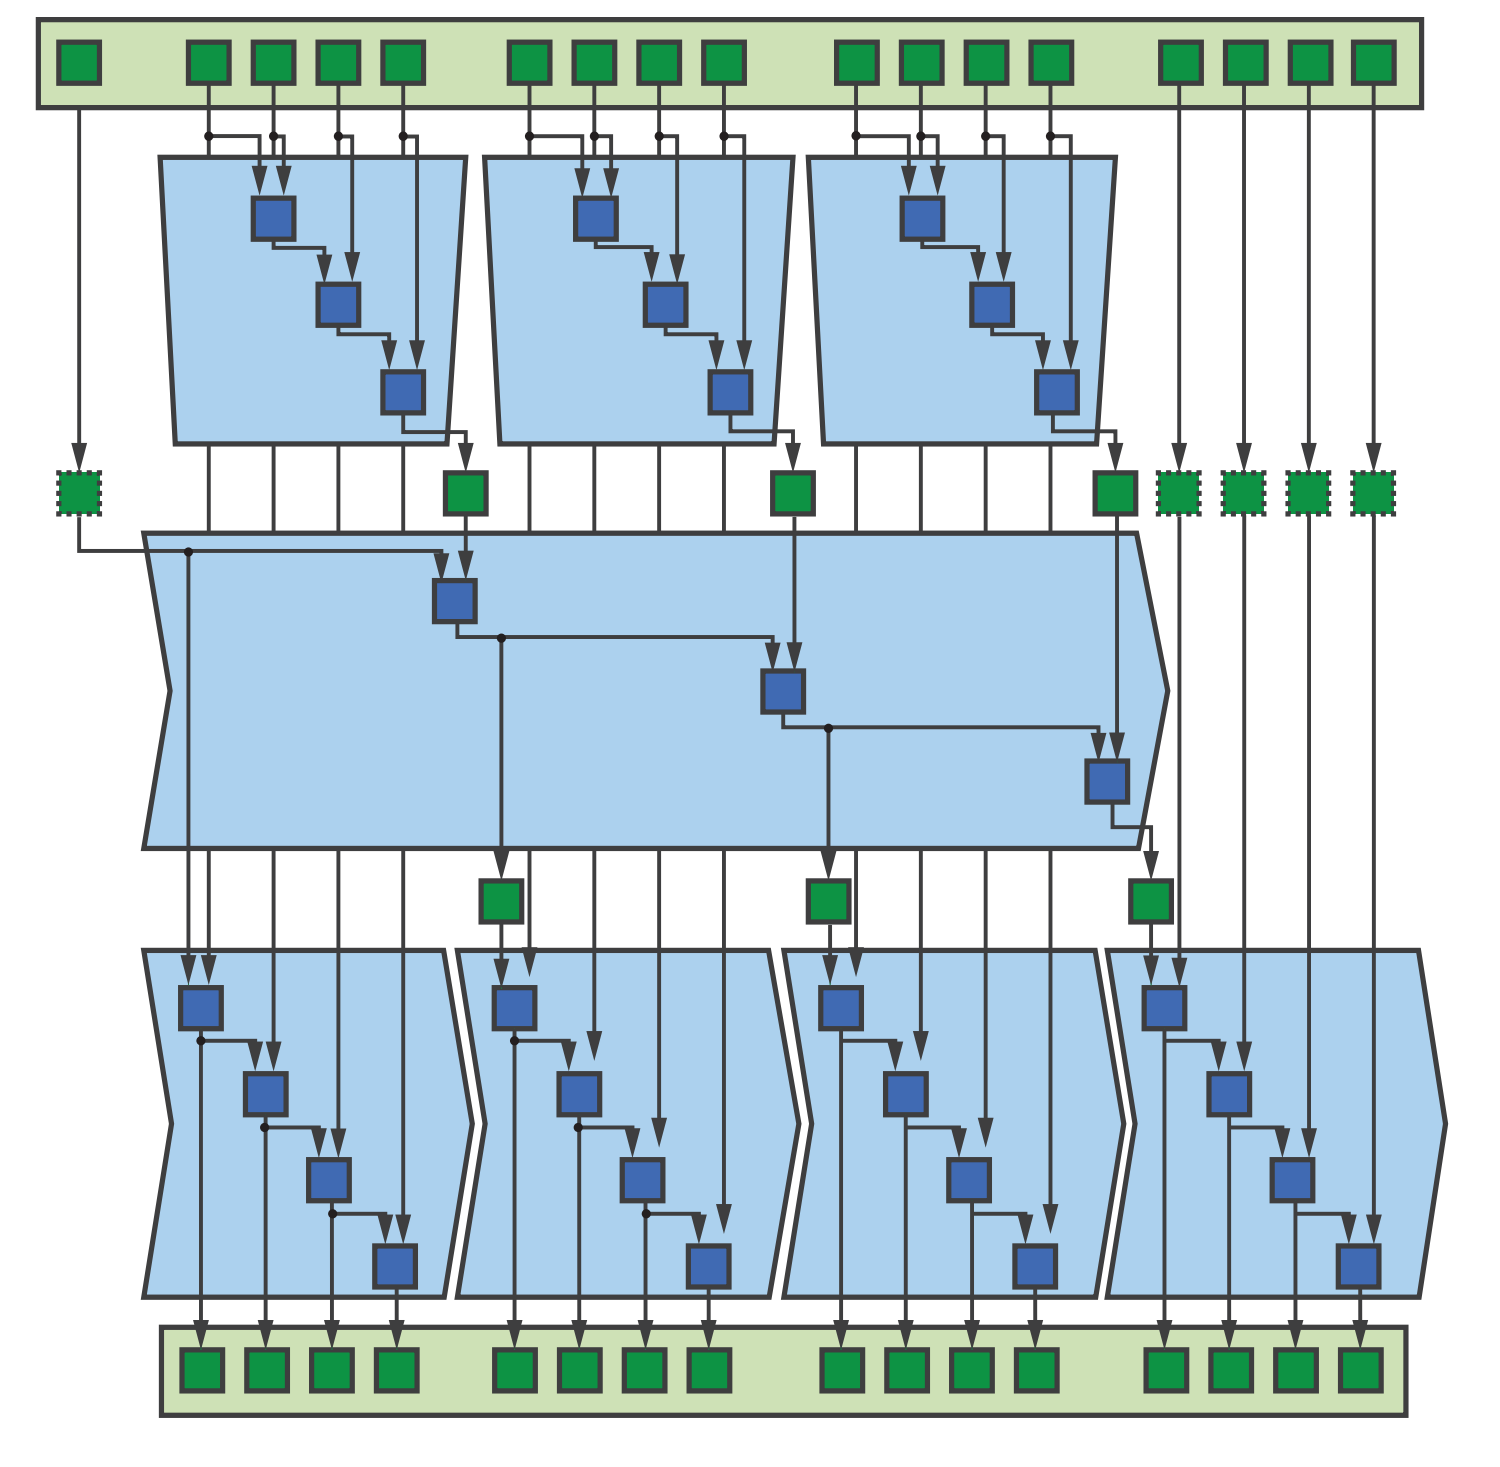
\includegraphics[width=1.\textwidth]{content/chapter-14/images/5}
\end{center}

Because the opportunities for parallelism within a scan operation are limited, the best device on which to execute a scan is highly dependent on problem size: smaller problems are a better fit for a CPU, since only larger problems will contain enough data parallelism to saturate a GPU. Problem size is less of a concern for FPGAs and other spatial architectures, since scans naturally lend themselves to pipeline parallelism. As in the case of a reduction, a good rule of thumb is to execute the scan operation on the same device that produced the data—considering where and how scan operations fit into an application during optimization will typically produce better results than focusing on optimizing the scan operations in isolation.\par

\hspace*{\fill} \par %插入空行
\textbf{Pack and Unpack}

The pack and unpack patterns are closely related to scans and are often implemented on top of scan functionality. We cover them separately here because they enable performant implementations of common operations (e.g., appending to a list) that may not have an obvious connection to prefix sums.\par

\hspace*{\fill} \par %插入空行
\textbf{Pack}

The pack pattern, shown in Figure 14-6, discards elements of an input range based on a Boolean condition, packing the elements that are not discarded into contiguous locations of the output range. This Boolean condition could be a pre-computed mask or could be computed online by applying some function to each input element.\par

\hspace*{\fill} \par %插入空行
Figure 14-6. Pack pattern
\begin{center}
	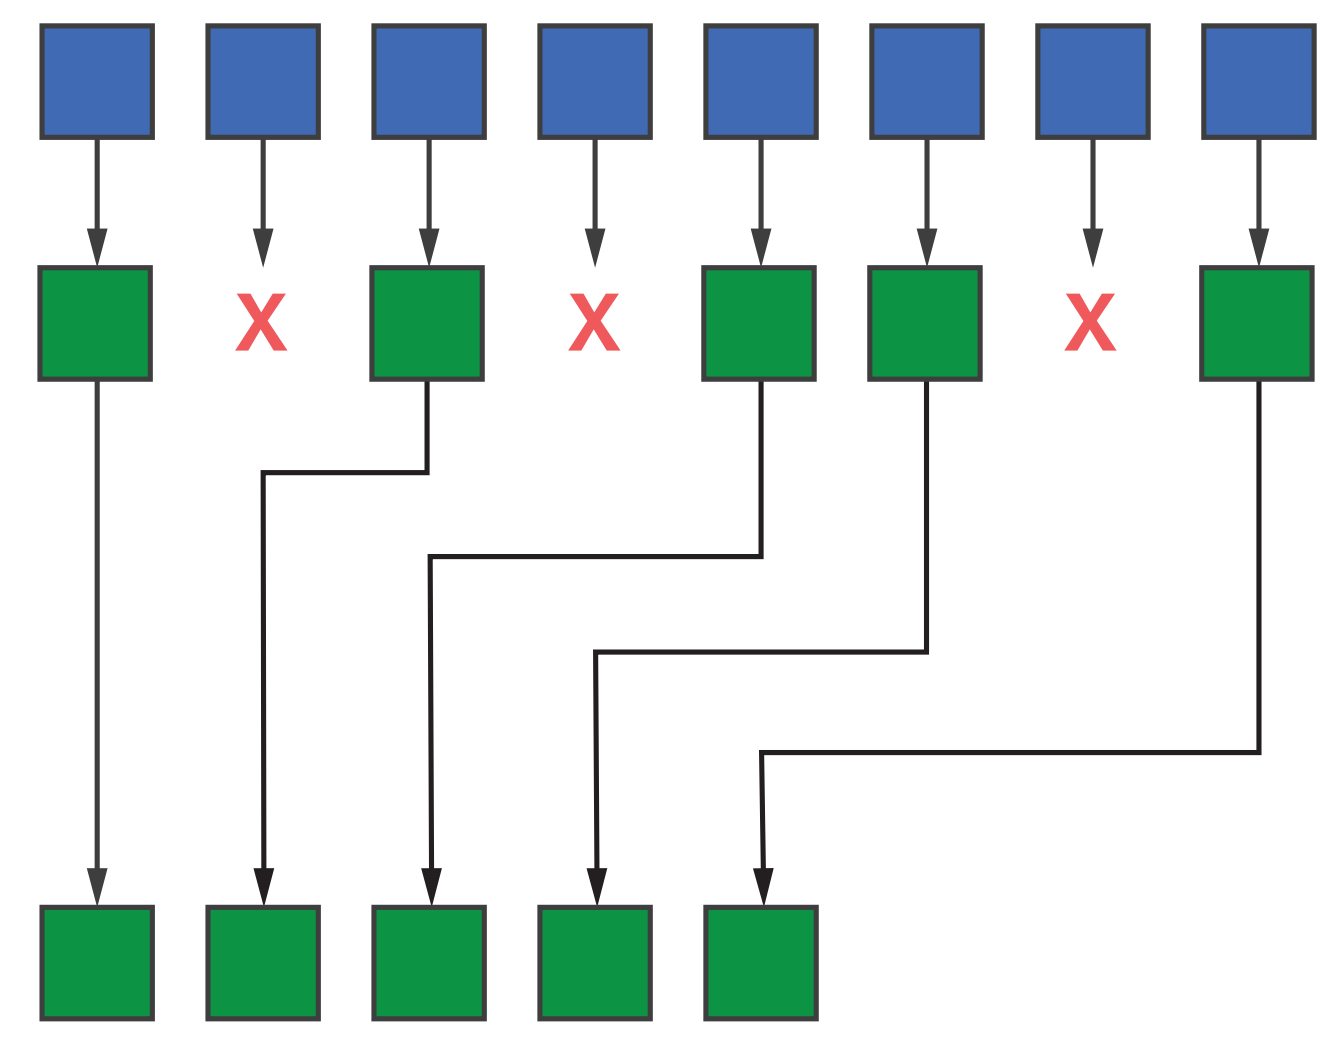
\includegraphics[width=1.\textwidth]{content/chapter-14/images/6}
\end{center}

Like with scan, there is an inherently serial nature to the pack operation. Given an input element to pack/copy, computing its location in the output range requires information about how many prior elements were also packed/copied into the output. This information is equivalent to an exclusive scan over the Boolean condition driving the pack.\par

\hspace*{\fill} \par %插入空行
\textbf{Unpack}

As shown in Figure 14-7 (and as its name suggests), the unpack pattern is the opposite of the pack pattern. Contiguous elements of an input range are unpacked into non-contiguous elements of an output range, leaving other elements untouched. The most obvious use case for this pattern is to unpack data that was previously packed, but it can also be used to fill in “gaps” in data resulting from some previous computation.\par

\hspace*{\fill} \par %插入空行
Figure 14-7. Unpack pattern
\begin{center}
	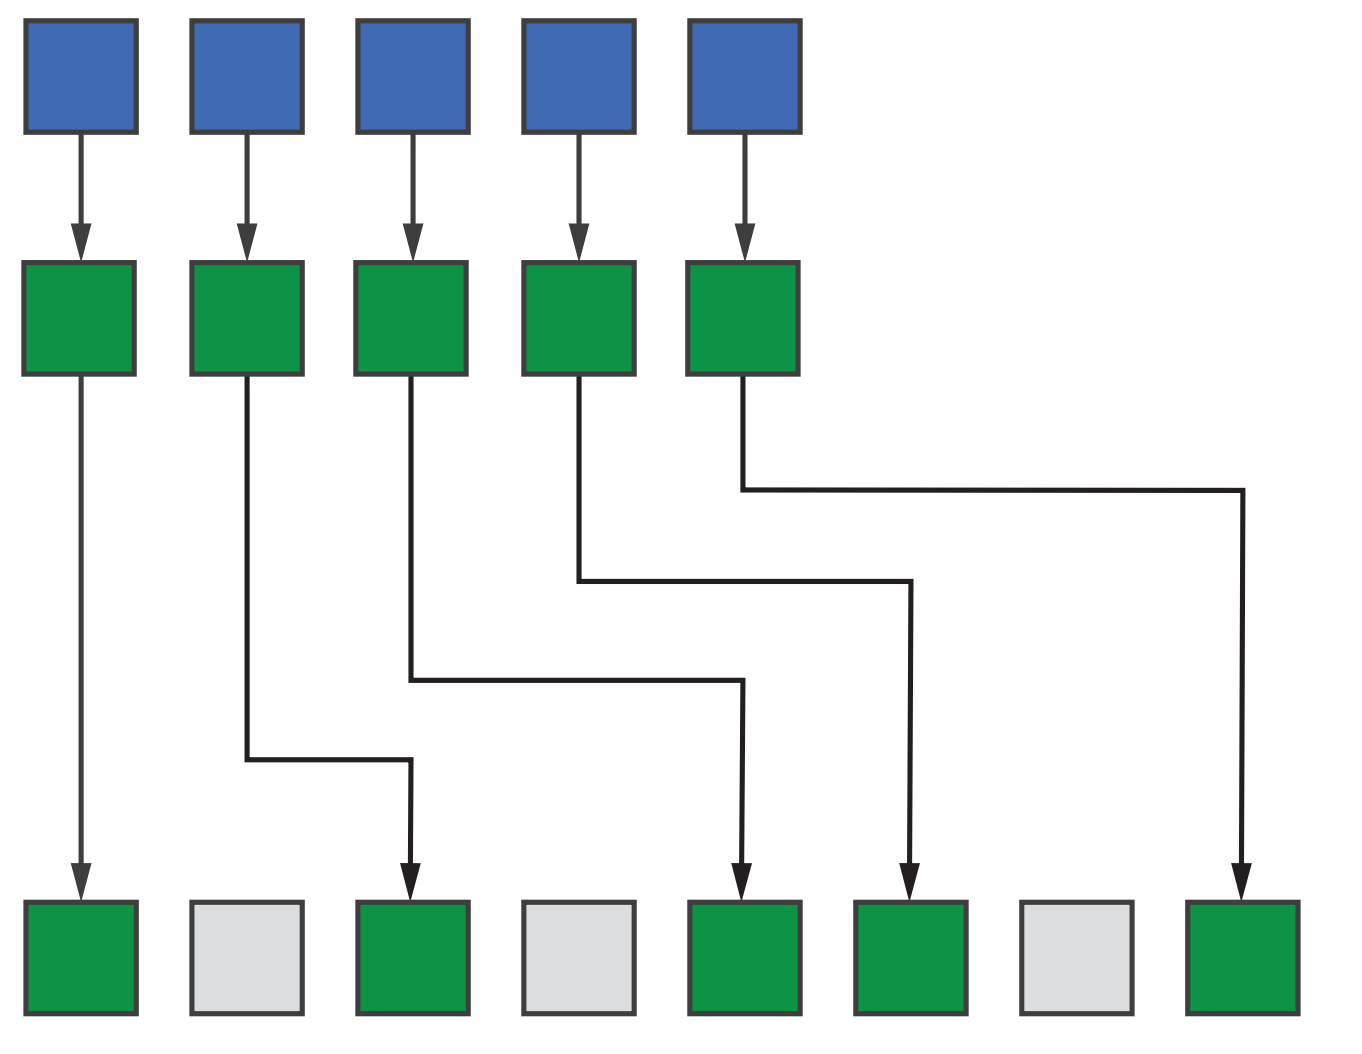
\includegraphics[width=1.\textwidth]{content/chapter-14/images/7}
\end{center}


















